%! Author = felix
%! Date = 14.10.2024

% Preamble
\documentclass[11pt]{article}

% Packages
\usepackage{amsmath}
\usepackage{amsfonts}
\usepackage{graphicx}

% Document
\begin{document}

\title{Übungsblatt 4}
\author{Felix Kleine Bösing, Juri Ernesto Humberg, Leonhard Meyer}
\maketitle

\section*{Aufgabe 1}

Bestimmen Sie alle komplexen Zahlen \( z = x + iy \in \mathbb{C} \) (\( x, y \in \mathbb{R} \)) mit \( z^3 = 1 \). Sie müssen beweisen, dass Sie keine Lösungen übersehen haben. Zeichnen Sie Ihre Lösungen im \( \mathbb{R}^2 \).

\subsection*{Berechnung der möglichen Lösungen}

\textbf{Beweis:}
Um alle komplexen Zahlen \( z = x + iy \) zu finden, für die \( z^3 = 1 \) gilt, gehen wir wie folgt vor:
\begin{enumerate}
    \item Zunächst schreiben wir \( z^3 = 1 \) in der Form:
    \[
    (x + iy)^3 = 1
    \]
    \item Entwickeln wir \( (x + iy)^3 \) mithilfe des Binomischen Satzes:
    \[
    (x + iy)^3 = x^3 + 3x^2(iy) + 3x(iy)^2 + (iy)^3
    \]
    \[
    = x^3 + 3x^2 \cdot iy + 3x \cdot (i^2 \cdot y^2) + (i^3 \cdot y^3)
    \]
    \item Da \( i^2 = -1 \) und \( i^3 = -i \), vereinfacht sich der Ausdruck zu:
    \[
    = x^3 + 3x^2 \cdot iy - 3x \cdot y^2 - iy^3
    \]
    \item Gruppieren wir nun die Real- und Imaginärteile:
    \[
    = (x^3 - 3xy^2) + i(3x^2y - y^3)
    \]
    \item Damit \( z^3 = 1 \) ist, muss der Realteil \( x^3 - 3xy^2 = 1 \) und der Imaginärteil \( 3x^2y - y^3 = 0 \) sein. Wir haben also das Gleichungssystem:
    \[
    x^3 - 3xy^2 = 1
    \]
    \[
    3x^2y - y^3 = 0
    \]
    \item Betrachten wir die zweite Gleichung \( 3x^2y - y^3 = 0 \). Diese können wir umformen zu:
    \[
    y(3x^2 - y^2) = 0
    \]
    Das liefert zwei Möglichkeiten:
    \begin{enumerate}
        \item \( y = 0 \): Wenn \( y = 0 \), wird \( z = x \) reell. Setzen wir \( y = 0 \) in die erste Gleichung ein, erhalten wir \( x^3 = 1 \), was \( x = 1 \) ergibt. Also ist eine Lösung \( z = 1 \).
        \item \( 3x^2 = y^2 \): Wenn \( y \neq 0 \), dann gilt \( y^2 = 3x^2 \), also \( y = \pm \sqrt{3}x \).
    \end{enumerate}
    \item Setzen wir \( y = \pm \sqrt{3}x \) in die erste Gleichung ein:
    \[
    x^3 - 3x(\pm \sqrt{3}x)^2 = 1
    \]
    \[
    x^3 - 3x \cdot 3x^2 = 1
    \]
    \[
    x^3 - 9x^3 = 1
    \]
    \[
    -8x^3 = 1 \Rightarrow x^3 = -\frac{1}{8} \Rightarrow x = -\frac{1}{2}
    \]
    \item Damit sind die möglichen Werte von \( x \) und \( y \):
    \[
    x = 1, \quad y = 0 \Rightarrow z = 1
    \]
    \[
    x = -\frac{1}{2}, \quad y = \pm \frac{\sqrt{3}}{2} \Rightarrow z = -\frac{1}{2} \pm i\frac{\sqrt{3}}{2}
    \]
\end{enumerate}

\textbf{Ergebnis:} Die Lösungen sind also:
\[
z_0 = 1, \quad z_1 = -\frac{1}{2} + i\frac{\sqrt{3}}{2}, \quad z_2 = -\frac{1}{2} - i\frac{\sqrt{3}}{2}
\]

\clearpage

\subsection*{Visualisierung in \(R^2\)}

Wir stellen die drei Punkte, die wir gefunden haben im Koordinatensystem dar. Diese liegen auf dem Einheitskreis
mit Radius 1.

\begin{figure}[h]
    \centering
    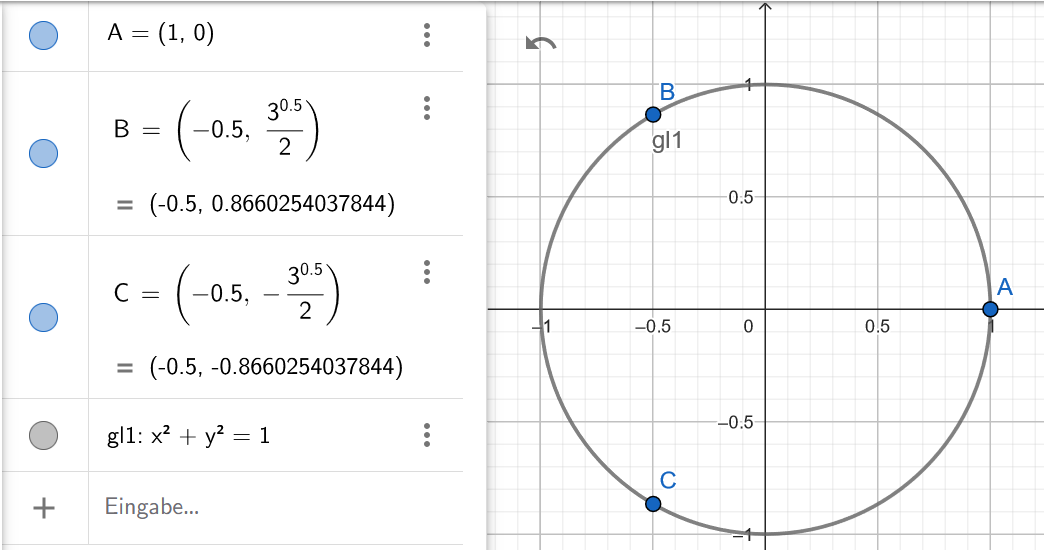
\includegraphics[width=0.75\textwidth]{img/a1_4_1.png}
    \caption{Darstellung der Lösungen im \(\mathbb{R}^2\)}
\end{figure}

\section*{Aufgabe 2}

Sei \( (z_n)_{n \in \mathbb{N}} \) eine komplexe Zahlenfolge mit
\[
z_n := i^n + \frac{1}{2} \left( \frac{1 + i}{\sqrt{2}} \right)^n
\]
für alle \( n \in \mathbb{N} \). Bestimmen Sie:

\begin{enumerate}
    \item[(a)] \( \sup(\{\operatorname{Re}(z_n) : n \in \mathbb{N}\}) \).
    \item[(b)] \( \inf(\{\operatorname{Im}(z_n) : n \in \mathbb{N}\}) \).
    \item[(c)] \( \sup(\{|z_n| : n \in \mathbb{N}\}) \).
\end{enumerate}

\subsection*{Lösung:}

Um die Teilaufgaben zu lösen, analysieren wir zunächst den Ausdruck für \( z_n \).

\subsection*{Teil (a)}

Betrachten wir den Realteil von \( z_n \):
\[
z_n = i^n + \frac{1}{2} \left( \frac{1 + i}{\sqrt{2}} \right)^n
\]

1. Der Term \( i^n \) wechselt periodisch in den Werten \( i^0 = 1 \), \( i^1 = i \), \( i^2 = -1 \), \( i^3 = -i \), und wiederholt sich dann alle vier Schritte. Somit hat der Realteil von \( i^n \) die Werte \( 1 \) und \( -1 \), abhängig davon, ob \( n \) gerade oder ungerade ist.

2. Der Ausdruck \( \frac{1 + i}{\sqrt{2}} \) hat den Betrag \( 1 \) und Argument \( \frac{\pi}{4} \). Somit ist \( \left( \frac{1 + i}{\sqrt{2}} \right)^n \) eine Drehung um den Ursprung und oszilliert im Einheitskreis. Der Realteil von \( \frac{1}{2} \left( \frac{1 + i}{\sqrt{2}} \right)^n \) oszilliert daher ebenfalls zwischen \( -\frac{1}{2} \) und \( \frac{1}{2} \).

Daraus folgt:
\[
\operatorname{Re}(z_n) \in \left[ -1 - \frac{1}{2}, 1 + \frac{1}{2} \right] = [-1.5, 1.5]
\]
und daher ist
\[
\sup(\{\operatorname{Re}(z_n) : n \in \mathbb{N}\}) = 1.5.
\]

\subsection*{Teil (b)}

Für den Imaginärteil von \( z_n \) gilt analog:

1. Der Imaginärteil von \( i^n \) wechselt periodisch in den Werten \( 0 \), \( 1 \), \( 0 \), \( -1 \), ebenfalls abhängig von \( n \) modulo 4.

2. Der Imaginärteil von \( \frac{1}{2} \left( \frac{1 + i}{\sqrt{2}} \right)^n \) oszilliert zwischen \( -\frac{1}{2} \) und \( \frac{1}{2} \).

Daraus ergibt sich:
\[
\operatorname{Im}(z_n) \in \left[ -1 - \frac{1}{2}, 1 + \frac{1}{2} \right] = [-1.5, 1.5]
\]
und daher ist
\[
\inf(\{\operatorname{Im}(z_n) : n \in \mathbb{N}\}) = -1.5.
\]

\subsection*{Teil (c)}

Betrachten wir den Betrag von \( z_n \):
\[
|z_n| = \left| i^n + \frac{1}{2} \left( \frac{1 + i}{\sqrt{2}} \right)^n \right|
\]

Da \( i^n \) und \( \frac{1}{2} \left( \frac{1 + i}{\sqrt{2}} \right)^n \) beide Beträge höchstens 1 haben, gilt:
\[
|z_n| \leq |i^n| + \left| \frac{1}{2} \left( \frac{1 + i}{\sqrt{2}} \right)^n \right| = 1 + \frac{1}{2} = 1.5
\]

Somit ist
\[
\sup(\{|z_n| : n \in \mathbb{N}\}) = 1.5.
\]

\textbf{Ergebnis:} Die gesuchten Werte sind:
\begin{enumerate}
    \item[(a)] \( \sup(\{\operatorname{Re}(z_n) : n \in \mathbb{N}\}) = 1.5 \)
    \item[(b)] \( \inf(\{\operatorname{Im}(z_n) : n \in \mathbb{N}\}) = -1.5 \)
    \item[(c)] \( \sup(\{|z_n| : n \in \mathbb{N}\}) = 1.5 \)
\end{enumerate}

\section*{Aufgabe 3}

Sei \( (a_n)_{n \in \mathbb{N}} \) eine Folge in \( \mathbb{R} \) mit \( a_n \to 0 \) und \( a_n > 0 \) für alle \( n \in \mathbb{N} \). Zeigen Sie, dass die Menge \( \{a_n \mid n \in \mathbb{N}\} \) ein Maximum besitzt. Zeigen Sie auch, dass die Menge \( \{a_n \mid n \in \mathbb{N}\} \) nicht notwendigerweise ein Maximum besitzt, falls nicht gefordert wird, dass \( a_n > 0 \) für jedes \( n \in \mathbb{N} \) gilt.

\subsection*{Lösung:}

\subsection*{Teil (a): Die Menge \( \{a_n \mid n \in \mathbb{N}\} \) besitzt ein Maximum, wenn \( a_n > 0 \) für alle \( n \in \mathbb{N} \)}

\textbf{Beweis:}
Da \( (a_n) \) eine konvergente Folge ist und \( a_n \to 0 \), folgt, dass die Folge eine obere Schranke besitzt, d.h., es existiert ein \( M > 0 \), sodass \( a_n \leq M \) für alle \( n \in \mathbb{N} \). Da \( a_n > 0 \) für alle \( n \in \mathbb{N} \), handelt es sich bei der Menge \( \{a_n \mid n \in \mathbb{N}\} \) um eine Teilmenge von \( (0, M] \), die nach oben beschränkt ist.

Da \( a_n \to 0 \) und \( a_n > 0 \) für alle \( n \in \mathbb{N} \), können wir schließen, dass die Folge von Werten \( \{a_n \mid n \in \mathbb{N}\} \) am Anfang größere Werte annimmt und sich dann gegen 0 bewegt. Somit existiert ein Index \( N \in \mathbb{N} \), für den \( a_N = \sup(\{a_n \mid n \in \mathbb{N}\}) \), da die Folge aufgrund der Konvergenz gegen 0 von einem Maximum ausgehend immer kleiner wird.

Damit besitzt die Menge \( \{a_n \mid n \in \mathbb{N}\} \) ein Maximum.

\subsection*{Teil (b): Die Menge \( \{a_n \mid n \in \mathbb{N}\} \) besitzt nicht notwendigerweise ein Maximum, wenn \( a_n > 0 \) für alle \( n \in \mathbb{N} \) nicht gefordert wird}

\textbf{Beweis:}
Wenn die Bedingung \( a_n > 0 \) für alle \( n \in \mathbb{N} \) entfällt, könnte die Folge \( (a_n) \) negative oder wechselnde Vorzeichen annehmen. Ein Beispiel für eine solche Folge ist \( a_n = (-1)^n + \frac{1}{n} \).

1. In diesem Fall konvergiert \( a_n \) ebenfalls gegen 0, aber die Werte der Folge oszillieren und erreichen kein Maximum.
2. Da die Folge \( a_n = (-1)^n + \frac{1}{n} \) abwechselnd positive und negative Werte annimmt, ist die Menge \( \{a_n \mid n \in \mathbb{N}\} \) nicht nach oben beschränkt und besitzt daher kein Maximum.

Dieses Beispiel zeigt, dass die Bedingung \( a_n > 0 \) für alle \( n \in \mathbb{N} \) entscheidend dafür ist, dass die Menge \( \{a_n \mid n \in \mathbb{N}\} \) ein Maximum besitzt. Ohne diese Bedingung könnte die Folge wechselnde Vorzeichen oder auch negative Werte annehmen, was dazu führt, dass die Menge kein Maximum besitzt.

\textbf{Ergebnis:}
\begin{enumerate}
    \item Die Menge \( \{a_n \mid n \in \mathbb{N}\} \) besitzt ein Maximum, wenn \( a_n > 0 \) für alle \( n \in \mathbb{N} \).
    \item Die Menge \( \{a_n \mid n \in \mathbb{N}\} \) besitzt nicht notwendigerweise ein Maximum, wenn die Bedingung \( a_n > 0 \) für alle \( n \in \mathbb{N} \) nicht gegeben ist.
\end{enumerate}

\section*{Aufgabe 4}

Untersuchen Sie die folgende Folgen auf Konvergenz beziehungsweise Divergenz.

\subsection*{Teil (a): \( (a_n)_{n \in \mathbb{N}} \) mit \( a_n := (-1)^n \)}

\textbf{Lösung:} Die Folge \( a_n = (-1)^n \) oszilliert zwischen den Werten \( 1 \) und \( -1 \), je nachdem, ob \( n \) gerade oder ungerade ist. Da die Folge keine feste Zahl als Grenzwert hat, ist sie divergent.

\[
\lim_{n \to \infty} a_n \text{ existiert nicht} \Rightarrow (a_n) \text{ ist divergent.}
\]

\subsection*{Teil (b): \( (b_n)_{n \in \mathbb{N}} \) mit \( b_n := \frac{n^2}{n^3 + 1} \)}

\textbf{Lösung:} Um das Verhalten der Folge \( b_n = \frac{n^2}{n^3 + 1} \) für \( n \to \infty \) zu untersuchen, betrachten wir den höchsten Exponenten im Zähler und Nenner.

\[
b_n = \frac{n^2}{n^3 + 1} = \frac{n^2}{n^3 \left(1 + \frac{1}{n^3}\right)} = \frac{1}{n \left(1 + \frac{1}{n^3}\right)}
\]

Da \( \frac{1}{n} \to 0 \) für \( n \to \infty \), folgt:

\[
\lim_{n \to \infty} b_n = 0
\]

Also konvergiert die Folge \( (b_n) \) gegen 0.

\subsection*{Teil (c): \( (c_n)_{n \in \mathbb{N}} \) mit \( c_n := \frac{4n^2 - 6n}{n^2 + 1} \)}

\textbf{Lösung:} Wir untersuchen das Verhalten von \( c_n = \frac{4n^2 - 6n}{n^2 + 1} \) für \( n \to \infty \), indem wir den höchsten Exponenten im Zähler und Nenner betrachten.

\[
c_n = \frac{4n^2 - 6n}{n^2 + 1} = \frac{n^2 (4 - \frac{6}{n})}{n^2 (1 + \frac{1}{n^2})} = \frac{4 - \frac{6}{n}}{1 + \frac{1}{n^2}}
\]

Da \( \frac{6}{n} \to 0 \) und \( \frac{1}{n^2} \to 0 \) für \( n \to \infty \), ergibt sich:

\[
\lim_{n \to \infty} c_n = \frac{4 - 0}{1 + 0} = 4
\]

Also konvergiert die Folge \( (c_n) \) gegen 4.

\subsection*{Teil (d): \( (d_n)_{n \in \mathbb{N}} \) mit \( d_n := \frac{n^2 + 1}{3n} \)}

\textbf{Lösung:} Wir untersuchen das Verhalten von \( d_n = \frac{n^2 + 1}{3n} \) für \( n \to \infty \), indem wir den höchsten Exponenten im Zähler und Nenner betrachten.

\[
d_n = \frac{n^2 + 1}{3n} = \frac{n \cdot \left(n + \frac{1}{n}\right)}{3n} = \frac{n + \frac{1}{n}}{3} = \frac{n}{3} + \frac{1}{3n}
\]

Da der Term \( \frac{n}{3} \to \infty \) für \( n \to \infty \), divergiert die Folge \( (d_n) \) gegen \( \infty \).

\[
\lim_{n \to \infty} d_n = \infty \Rightarrow (d_n) \text{ ist divergent.}
\]

\subsection*{Ergebnis:}
\begin{enumerate}
    \item[(a)] Die Folge \( (a_n) = (-1)^n \) ist divergent.
    \item[(b)] Die Folge \( (b_n) = \frac{n^2}{n^3 + 1} \) konvergiert gegen 0.
    \item[(c)] Die Folge \( (c_n) = \frac{4n^2 - 6n}{n^2 + 1} \) konvergiert gegen 4.
    \item[(d)] Die Folge \( (d_n) = \frac{n^2 + 1}{3n} \) ist divergent gegen \( \infty \).
\end{enumerate}



\end{document}
